\documentclass[a4paper,11pt]{article}
\usepackage[spanish]{babel}
\usepackage[utf8]{inputenc}

% Configuración páginas
\usepackage{vmargin}				% Márgenes

\usepackage{sectsty}				% Fuente de los títulos
\allsectionsfont{\normalfont \Large \scshape}

\usepackage{graphicx}				% Imágenes
\graphicspath{{images/}}

\usepackage{mathtools}				% Matematicas
\newcommand\tab[1][1cm]{\hspace*{#1}}	% Un tabulador

% Configuración del título
\newcommand{\horrule}[1]{\rule{\linewidth}{#1}} 	% Horizontal rule

\title{
	\vspace{-25pt}
	\normalfont \Large \textsc{
		Minería de Datos, Ingeniería Informática\\
		Universidad de Valladolid
	}\\[10pt]
	\horrule{1pt}\\[10pt]
	\huge \textbf{
		Práctica de redes neuronales para predicción
	}\\
	\horrule{1pt}
}
\author{
	\normalfont \Large Daniel González Alonso
}
\date{
	\normalfont \large \today
}

%%%%%%%%%%%%%%%%%%%%%%%%%%%%%%%%%%%%%%%%%%%%%%%%%%
\begin{document}
\maketitle

\begin{abstract}
	En este documento se describen las fases hacia adelante y hacia atrás de las redes de Elman y Jordan, así como la evolución de la tasa de aciertos en la predicción de la cotización de Iberdrola para la práctica de redes neuronales para predicción de la asignatura Minería de Datos de Ingeniería Informática, Universidad de Valladolid.
\end{abstract}

%%%% INTRODUCCIÓN %%%%
\section{Introducción}
En este documento primero se describirá la Red de Elman y después la Red de Jordan, en ambos casos se incluirá apartados con la fase hacia adelante y hacia atrás así como los resultados obtenidos en la implementación de estas redes con Octave.\\

Antes de empezar voy a aclarar las posibles dudas que haya con la notación utilizada:

\begin{itemize}
	\item Para la función de activación emplearé siempre el símbolo ${F(x)}$, en mi caso se ha empleado la función sigmoide ${F(x) = \frac{1}{1+e^{-x}}}$ tanto para la capa de salida como para la capa oculta.

	\item El vector ${y(t)}$ siempre se va a referir a los valores obtenidos por una de las capas de la red neuronal en el instante ${t}$, mientras que ${x(t)}$ representará a los valores de entrada a la red neuronal en el instante ${t}$.

	\item ${NI}$ representará el número de neuronas de entrada, ${N0}$ el número de neuronas de la capa oculta, y ${N1}$ representará el número de neuronas de la capa de salida.
    
    \item ${w_{i,j}}$ se refiere al peso de la conexión entre una neurona ${j}$ a la neurona ${i}$.

	\item Un superíndice 1, ya sea en ${y(t)}$ o en ${w_{i,j}}$, siempre se referirá a la capa de salida, mientras que un superíndice 0 se referirá a la capa oculta.
\end{itemize}

%%%% DESARROLLO %%%%
\newpage
% RED DE ELMAN
\section{Red de Elman}

\begin{figure}[!htbp]
	\centering
	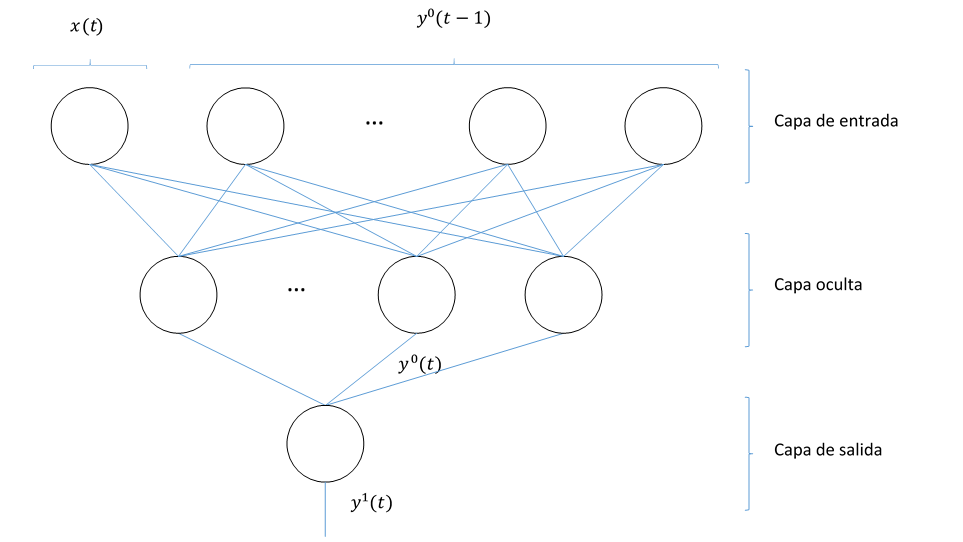
\includegraphics[width=1.0\textwidth]{red_elman.png}
\end{figure}

\subsection{Fase hacia delante}
En esta fase se calculará las salidas de la red neuronal de Elman en el instante ${t}$. Hay que tener en cuenta de que tratamos de una serie temporal en la que dependemos de los ${\tau}$ valores anteriores y del valor actual de ${x_{i}(t)}$ (solo un valor de ${x}$) para predecir el siguiente valor de ${y_{i}^{1}(t)}$ (solo un valor de ${y^{1}}$). Como en la red implementada solo hay dos capas tal y como se ve en el dibujo anterior, voy a dividir los cálculos de esta fase en la capa de salida y en la capa oculta.

\subsubsection{Capa de salida}
Los valores obtenidos por la capa de salida en la iteración ${t}$ se calculan con la siguiente fórmula:

\begin{equation}
	\label{elman_salida_y}
	y_{i}^{1}(t) = F\left(u_{i}^{1}(t)\right)
\end{equation}

Donde ${y_{i}^{1}(t)}$ representa el valor obtenido por la neurona ${i}$ de la capa de salida en el instante ${t}$. Por otro lado ${u_{i}^{1}(t)}$ representa el sumatorio de los valores de entrada de la neurona ${i}$ después de aplicar sus respectivos pesos, el cual se calcula mediante la siguiente fórmula:

\begin{equation}
	\label{salida_u}
	u_{i}^{1}(t) = \sum_{j=1}^{N0}{w_{i,j}^{1} \cdot y_{j}^{0}(t)} + w_{i,N0+1}^{1}
\end{equation}

Donde ${w_{i,j}^{1}}$ representa el peso de la conexión de la neurona ${j}$ de la capa oculta a la neurona ${i}$ de la capa de salida, e ${y_{j}^{0}(t)}$ representa la salida de la neurona ${j}$ de la capa oculta en el instante ${t}$. El último término ${w_{i,N0+1}^{1}}$ representa el peso del factor \textit{bias} de la red neuronal.

\subsubsection{Capa oculta}
Los valores obtenidos por la capa oculta en la iteración ${t}$ se calculan con la siguiente fórmula:

\begin{equation}
	y_{j}^{0}(t) = F\left(u_{j}^{0}(t)\right)
\end{equation}

Donde ${y_{j}^{0}(t)}$ representa el valor obtenido por la neurona ${j}$ de la capa oculta en el instante ${t}$, ${u_{j}^{0}(t)}$ es la suma de los valores de entrada de la neurona ${j}$ junto con los valores obtenidos en la iteración anterior después de aplicar sus respectivos pesos, el cual se calcula mediante la siguiente fórmula:

\begin{equation}
	\label{elman_oculta_u}
	u_{j}^{0}(t) = \sum_{k=1}^{NI}{w_{j,k}^{0} \cdot x_{k}(t)} + \sum_{k=NI+1}^{NI+N0}{w_{j,k}^{0} \cdot y_{k-NI}^{0}(t-1)} + w_{j,NI+N0+1}
\end{equation}

Donde ${w_{j,k}^{0}}$ en el primer sumatorio representa el peso de la conexión de la neurona ${k}$ de la capa de entrada a la neurona ${j}$ de la capa oculta, ${x_{k}(t)}$ representa la entrada en el instante actual, ${w_{j,k}^{0}}$ en el segundo sumatorio es el peso de la conexión entre la neurona ${k}$ con la neurona ${j}$, ambas de la capa oculta, y por último ${y_{k-NI}^{0}(t-1)}$ representa la salida de la neurona ${k-NI}$ de la capa oculta en el instante ${t-1}$ (la iteración anterior).

\subsection{Fase hacia atrás}
El objetivo de esta fase es calcular las variaciones que han de llevarse a cabo sobre cada peso de la red neuronal a partir de una función de error ${E(t)}$. Esta función de error en mi caso la he calculado como la distancia euclídea entre la salida esperada para una entrada y la predicha en el instante anterior, con lo cual la función es la siguiente:

\begin{equation}
	E(t) = \frac{1}{2}\sum_{i=1}^{N1}\left(x_{i}(t) - y_{i}^{1}(t-1)\right)^{2}
\end{equation}

Para el calculo de de la variación que ha de sufrir cada peso, se emplea la siguiente fórmula: 

\begin{equation}
	\label{elman_variacion_delta}
	\Delta w_{i,j}(t) = -\alpha \cdot \frac{\partial E(t)}{\partial w_{i,j}}
\end{equation}

Donde ${\alpha}$ es el ratio de aprendizaje elegido. Para calcular ${\Delta w_{i,j}(t)}$ vamos a dividir esta fase de nuevo en la capa de salida y la capa oculta.

\subsubsection{Capa de salida}
Para calcular la variación en los pesos de la neurona ${i}$ de la capa de salida, ${\Delta w_{i,j}^{1}(t)}$, primero hemos de calcular ${\frac{\partial E(t)}{\partial w_{i,j}^{1}}}$. Aplicando la regla de la cadena se obtiene:

\begin{equation}
	\frac{\partial E(t)}{\partial w_{i,j}^{1}} = \frac{\partial E(t)}{\partial y_{i}^{1}(t-1)} \cdot \frac{\partial y_{i}^{1}(t-1)}{\partial u_{i}^{1}(t-1)} \cdot \frac{\partial u_{i}^{1}(t-1)}{\partial w_{i,j}^{1}}
\end{equation}

Donde el primer factor se calcula como:

\begin{equation}
	\label{elman_derivada_E}
	\frac{\partial E(t)}{\partial y_{i}^{1}(t-1)} = \frac{\partial}{\partial y_{i}^{1}(t-1)}\left(\frac{1}{2}\left(x_{i}(t)-y_{i}^{1}(t-1)\right)^{2}\right) = -\left(x_{i}(t) - y_{i}^{1}(t-1)\right)
\end{equation}

El segundo lo dejamos indicado como la derivada ${F'\left(u_{i}^{1}(t-1)\right)}$. Combinando tanto el primer factor como este segundo, tenemos como resultado la función:

\begin{equation}
	\delta_{i}^{1}(t) = -\left(x_{i}(t) - y_{i}^{1}(t-1)\right) \cdot F'\left(u_{i}^{1}(t-1)\right)
\end{equation}

Por último, el tercer factor es:

\textbf{\begin{equation}
	\frac{\partial u_{i}^{1}(t-1)}{\partial w_{i,j}^{1}} =
    \begin{dcases}
    	y_{j}^{0}(t-1)	& \textrm{si } j=1,...,N0\\
		1				& \textrm{si } j=N0+1\\
	\end{dcases}
\end{equation}}

Finalmente, para obtener la variación que hemos de llevar a cabo sobre el peso, ${\Delta w_{i,j}^{1}}$, mediante los resultados anteriores y la fórmula \ref{elman_variacion_delta}, obtenemos:

\begin{equation}
	\Delta w_{i,j}^{1}(t) = -\alpha \cdot \frac{\partial E(t)}{\partial w_{i,j}^{1}} =
    \begin{dcases}
    	-\alpha \cdot \delta_{i}^{1}(t) \cdot y_{j}^{0}(t-1)	& \textrm{si } j=1,...,N0\\
		-\alpha \cdot \delta_{i}^{1}(t)							& \textrm{si } j=N0+1\\
	\end{dcases}
\end{equation}

\subsubsection{Capa oculta}
Para calcular la variación en los pesos de la neurona ${j}$ de la capa oculta, ${\Delta w_{j,k}^{0}(t)}$, primero hemos de calcular ${\frac{\partial E(t)}{\partial w_{j,k}^{0}}}$. Una vez más, aplicando la regla de la cadena se obtiene:

\begin{equation}
	\label{elman_oculta_derivada_E}
	\frac{\partial E(t)}{\partial w_{j,k}^{0}} = \frac{\partial E(t)}{\partial y_{j}^{0}(t-1)} \cdot \frac{\partial y_{j}^{0}(t-1)}{\partial u_{j}^{0}(t-1)} \cdot \frac{\partial u_{j}^{0}(t-1)}{\partial w_{j,k}^{0}}
\end{equation}

El primer factor lo obtenemos aplicando de nuevo la regla de la cadena:

\begin{equation}
	\frac{\partial E(t)}{\partial y_{j}^{0}(t-1)} = \frac{\partial E(t)}{\partial y_{i}^{1}(t-1)} \cdot \frac{\partial y_{i}^{1}(t-1)}{\partial u_{i}^{1}(t-1)} \cdot \frac{\partial u_{i}^{1}(t-1)}{\partial y_{j}^{0}(t-1)}
\end{equation}

Donde el primer y segundo factor se habían calculado anteriormente en la capa de salida como ${\delta_{i}^{1}(t)}$ y el último da simplemente ${w_{i,j}^{1}}$.

Por otro lado, el segundo factor de la fórmula \ref{elman_oculta_derivada_E} da como resultado ${F'\left(u_{j}^{0}(t-1)\right)}$, si combinamos todo lo calculado hasta ahora tenemos:

\begin{equation}
	\delta_{j}^{0}(t) = \delta_{i}^{1}(t) \cdot w_{i,j}^{1} \cdot F'\left(u_{j}^{0}(t-1)\right)
\end{equation}

Para el último factor de la fórmula \ref{elman_oculta_derivada_E}, tenemos que:

\begin{equation}
	\frac{\partial u_{j}^{0}(t-1)}{\partial w_{j,k}^{0}} =
	\begin{dcases}
		x_{k}(t-1)			& \textrm{si } k=1,...,NI\\
		y_{k-NI}^{0}(t-2)	& \textrm{si } k=NI+1,...,NI+N0\\
		1					& \textrm{si } k=NI+N0+1
	\end{dcases}
\end{equation}

Finalmente, si lo juntamos todo para obtener la variación que hay que realizar sobre el peso ${\Delta w_{j,k}^{0}}$, obtenemos:

\begin{equation}
	\Delta w_{j,k}^{0} = -\alpha \cdot \frac{\partial E}{\partial w_{j,k}^{0}} =
    \begin{dcases}
		-\alpha \cdot \delta_{j}^{0}(t) \cdot x_{k}(t-1)
        	& \textrm{si } k=1,...,NI\\
		-\alpha \cdot \delta_{j}^{0}(t) \cdot y_{k-NI}^{0}(t-2)
        	& \textrm{si } k=NI+1,...,NI+N0\\
		-\alpha \cdot \delta_{j}^{0}(t)
        	& \textrm{si } k=NI+N0+1
	\end{dcases}
\end{equation}

\subsection{Resultados obtenidos}
El código de la red de Elman está implementado en el archivo \texttt{red\_elman.m} que acompaña a este texto, este fichero fue programado en Octave 4.0.3. Los datos empleados se encuentran en el archivo \texttt{iberdrola\_Nov15-Dic16.csv} y para la implementación se dividieron mediante \textit{Hold-Out} (2/3 entrenamiento - 1/3 prueba). La evolución de los resultados que se han ido obteniendo para el conjunto de prueba a lo largo de las iteraciones ha sido:

\begin{figure}[!htbp]
	\centering
	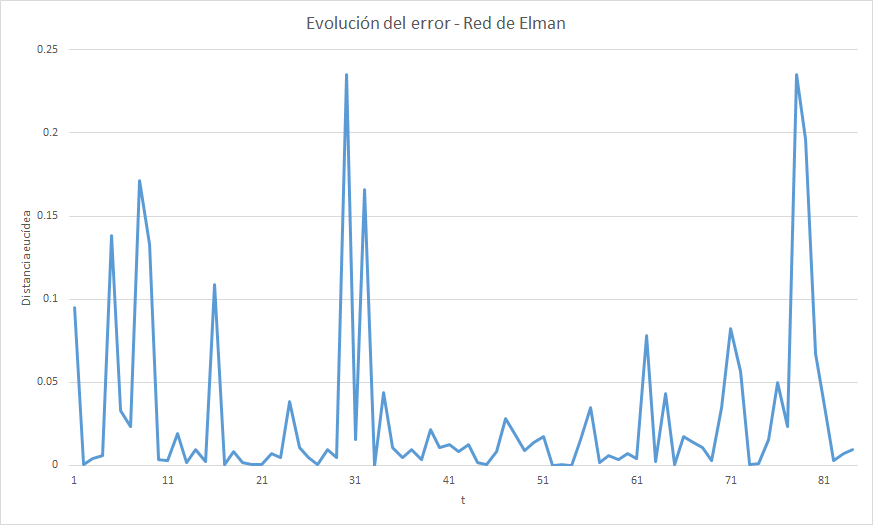
\includegraphics[width=1.0\textwidth]{red_elman_error.png}
\end{figure}

En este caso, teniendo en cuenta que un valor predicho se consideraba acierto si el error era inferior a 0.05, podemos concluir que más de un 75\% de los valores predichos son aciertos.

\newpage
% RED DE JORDAN
\section{Red de Jordan}

\begin{figure}[!htbp]
	\centering
	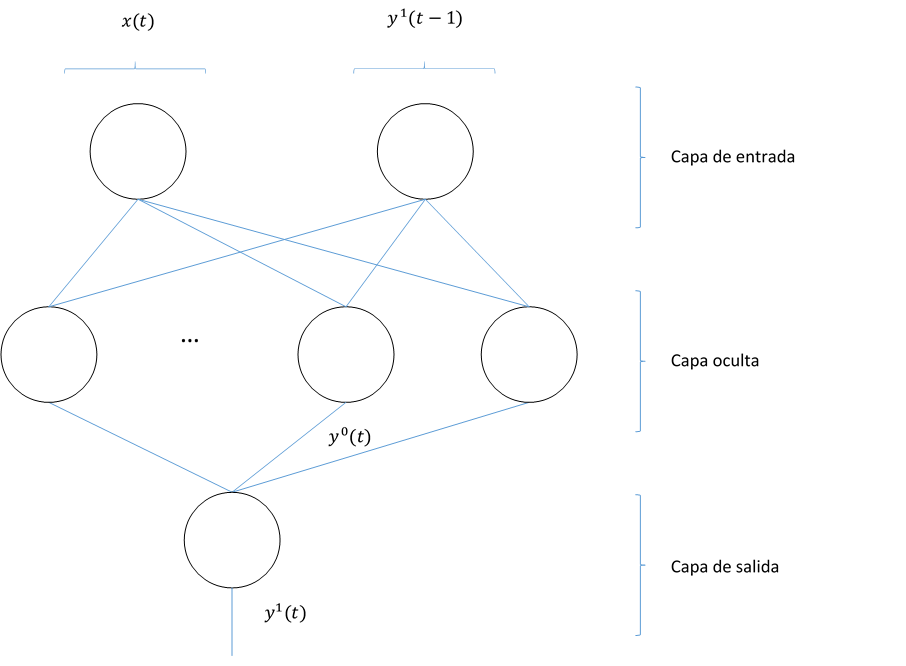
\includegraphics[width=1.0\textwidth]{red_jordan.png}
\end{figure}

\subsection{Fase hacia delante}
En esta fase se calculará las salidas de la red neuronal de Jordan en el instante ${t}$. En este caso tratamos de una serie temporal en la que dependemos únicamente del valor anterior ${y_{i}^{1}(t-1)}$ y de el valor actual de ${x_{i}(t)}$ (solo un valor de ${x}$) para predecir el siguiente valor de ${y_{i}^{1}(t)}$. Al igual que en la red de Elman, como en la red implementada solo hay dos capas tal y como se ve en el dibujo anterior, voy a dividir los cálculos de esta fase en la capa de salida y en la capa oculta.

\subsubsection{Capa de salida}
Los valores obtenidos por la capa de salida en la iteración ${t}$ se calculan con la siguiente fórmula:

\begin{equation}
	\label{jordan_salida_y}
	y_{i}^{1}(t) = F\left(u_{i}^{1}(t)\right)
\end{equation}

Donde ${y_{i}^{1}(t)}$ representa el valor obtenido por la neurona ${i}$ de la capa de salida en el instante ${t}$. Por otro lado ${u_{i}^{1}(t)}$ representa el sumatorio de los valores de entrada de la neurona ${i}$ después de aplicar sus respectivos pesos, el cual se calcula mediante la siguiente fórmula:

\begin{equation}
	\label{jordan_salida_u}
	u_{i}^{1}(t) = \sum_{j=1}^{N0}{w_{i,j}^{1} \cdot y_{j}^{0}(t)} + w_{i,N0+1}^{1}
\end{equation}

Donde ${w_{i,j}^{1}}$ representa el peso de la conexión de la neurona ${j}$ de la capa oculta a la neurona ${i}$ de la capa de salida, e ${y_{j}^{0}(t)}$ representa la salida de la neurona ${j}$ de la capa oculta en el instante ${t}$. El último término ${w_{i,N0+1}^{1}}$ representa el peso del factor \textit{bias} de la red neuronal.

\subsubsection{Capa oculta}
Los valores obtenidos por la capa oculta en la iteración ${t}$ se calculan con la siguiente fórmula:

\begin{equation}
	y_{j}^{0}(t) = F\left(u_{j}^{0}(t)\right)
\end{equation}

Donde ${y_{j}^{0}(t)}$ representa el valor obtenido por la neurona ${j}$ de la capa oculta en el instante ${t}$, ${u_{j}^{0}(t)}$ es la suma del valores de entrada de la neurona ${j}$ junto los valores obtenidos en la iteración anterior en la capa de salida después de aplicar sus respectivos pesos, el cual se calcula mediante la siguiente fórmula:

\begin{equation}
	\label{jordan_oculta_u}
	u_{j}^{0}(t) = \sum_{k=1}^{NI}w_{j,k}^{0} \cdot x_{k}(t) + \sum_{k=NI+1}^{NI+N1}{w_{j,k}^{0} \cdot y_{k-NI}^{1}(t-1)} + w_{j,NI+N0+1}
\end{equation}

Donde ${w_{j,k}^{0}}$ en el primer término representa el peso de la conexión de la neurona ${k}$ de la capa de entrada a la neurona ${j}$ de la capa oculta, ${x_{k}(t)}$ representa la entrada en el instante actual, en el segundo sumatorio, ${w_{j,k}^{0}}$ es el peso de la conexión entre la neurona ${k}$ de la capa de salida con la neurona ${j}$ de la capa oculta, y por último ${y_{k-NI}^{1}(t-1)}$ representa la salida de la neurona ${k-NI}$ de la capa de salida en el instante ${t-1}$ (la iteración anterior).

\subsection{Fase hacia atrás}
El objetivo de esta fase es calcular las variaciones que han de llevarse a cabo sobre cada peso de la red neuronal a partir de una función de error ${E(t)}$. Esta función de error se ha vuelto a calcular como la distancia euclídea entre la salida esperada para una entrada y la predicha en el instante anterior, con lo cual la función es la siguiente:

\begin{equation}
	E(t) = \frac{1}{2}\sum_{i=1}^{N1}\left(x_{i}(t) - y_{i}^{1}(t-1)\right)^{2}
\end{equation}

Para el cálculo de la variación que ha de sufrir cada peso, se emplea la siguiente fórmula: 

\begin{equation}
	\label{jordan_variacion_delta}
	\Delta w_{i,j}(t) = -\alpha \cdot \frac{\partial E(t)}{\partial w_{i,j}}
\end{equation}

Donde ${\alpha}$ es el ratio de aprendizaje elegido. Para calcular ${\Delta w_{i,j}(t)}$ vamos a dividir esta fase de nuevo en la capa de salida y la capa oculta.

\subsubsection{Capa de salida}
Para calcular la variación en los pesos de la neurona ${i}$ de la capa de salida, ${\Delta w_{i,j}^{1}(t)}$, primero hemos de calcular ${\frac{\partial E(t)}{\partial w_{i,j}^{1}}}$. Aplicando la regla de la cadena se obtiene:

\begin{equation}
	\frac{\partial E(t)}{\partial w_{i,j}^{1}} = \frac{\partial E(t)}{\partial y_{i}^{1}(t-1)} \cdot \frac{\partial y_{i}^{1}(t-1)}{\partial u_{i}^{1}(t-1)} \cdot \frac{\partial u_{i}^{1}(t-1)}{\partial w_{i,j}^{1}}
\end{equation}

Donde el primer factor se calcula como:

\begin{equation}
	\label{jordan_derivada_E}
	\frac{\partial E(t)}{\partial y_{i}^{1}(t-1)} = \frac{\partial}{\partial y_{i}^{1}(t-1)}\left(\frac{1}{2}\left(x_{i}(t)-y_{i}^{1}(t-1)\right)^{2}\right) = -\left(x_{i}(t) - y_{i}^{1}(t-1)\right)
\end{equation}

El segundo lo dejamos indicado como la derivada ${F'\left(u_{i}^{1}(t-1)\right)}$. Combinando tanto el primer factor como este segundo, tenemos como resultado la función:

\begin{equation}
	\delta_{i}^{1}(t) = -\left(x_{i}(t) - y_{i}^{1}(t-1)\right) \cdot F'\left(u_{i}^{1}(t-1)\right)
\end{equation}

Por último, el tercer factor es:

\textbf{\begin{equation}
	\frac{\partial u_{i}^{1}(t-1)}{\partial w_{i,j}^{1}} =
    \begin{dcases}
    	y_{j}^{0}(t-1)	& \textrm{si } j=1,...,N0\\
		1				& \textrm{si } j=N0+1\\
	\end{dcases}
\end{equation}}

Finalmente, para obtener la variación que hemos de llevar a cabo sobre el peso, ${\Delta w_{i,j}^{1}}$, mediante los resultados anteriores y la fórmula \ref{jordan_variacion_delta}, obtenemos:

\begin{equation}
	\Delta w_{i,j}^{1}(t) = -\alpha \cdot \frac{\partial E(t)}{\partial w_{i,j}^{1}} =
    \begin{dcases}
    	-\alpha \cdot \delta_{i}^{1}(t) \cdot y_{j}^{0}(t-1)	& \textrm{si } j=1,...,N0\\
		-\alpha \cdot \delta_{i}^{1}(t)							& \textrm{si } j=N0+1\\
	\end{dcases}
\end{equation}

\subsubsection{Capa oculta}
Para calcular la variación en los pesos de la neurona ${j}$ de la capa oculta, ${\Delta w_{j,k}^{0}(t)}$, primero hemos de calcular ${\frac{\partial E(t)}{\partial w_{j,k}^{0}}}$. Una vez más, aplicando la regla de la cadena se obtiene:

\begin{equation}
	\label{jordan_oculta_derivada_E}
	\frac{\partial E(t)}{\partial w_{j,k}^{0}} = \frac{\partial E(t)}{\partial y_{j}^{0}(t-1)} \cdot \frac{\partial y_{j}^{0}(t-1)}{\partial u_{j}^{0}(t-1)} \cdot \frac{\partial u_{j}^{0}(t-1)}{\partial w_{j,k}^{0}}
\end{equation}

El primer factor lo obtenemos aplicando de nuevo la regla de la cadena:

\begin{equation}
	\frac{\partial E(t)}{\partial y_{j}^{0}(t-1)} = \frac{\partial E(t)}{\partial y_{i}^{1}(t-1)} \cdot \frac{\partial y_{i}^{1}(t-1)}{\partial u_{i}^{1}(t-1)} \cdot \frac{\partial u_{i}^{1}(t-1)}{\partial y_{j}^{0}(t-1)}
\end{equation}

Donde el primer y segundo factor se habían calculado anteriormente en la capa de salida como ${\delta_{i}^{1}(t)}$ y el último da simplemente ${w_{i,j}^{1}}$.

Por otro lado, el segundo factor de la fórmula \ref{jordan_oculta_derivada_E} da como resultado ${F'\left(u_{j}^{0}(t-1)\right)}$, si combinamos todo lo calculado hasta ahora tenemos:

\begin{equation}
	\delta_{j}^{0}(t) = \delta_{i}^{1}(t) \cdot w_{i,j}^{1} \cdot F'\left(u_{j}^{0}(t-1)\right)
\end{equation}

Para el último factor de la fórmula \ref{jordan_oculta_derivada_E}, tenemos que:

\begin{equation}
	\frac{\partial u_{j}^{0}(t-1)}{\partial w_{j,k}^{0}} =
	\begin{dcases}
		x_{k}(t-1)			& \textrm{si } k=1,...,NI\\
		y_{k-NI}^{1}(t-2)	& \textrm{si } k=NI+1,...,NI+N1\\
		1					& \textrm{si } k=NI+N1+1
	\end{dcases}
\end{equation}

Finalmente, si lo juntamos todo para obtener la variación que hay que realizar sobre el peso ${\Delta w_{j,k}^{0}}$, obtenemos:

\begin{equation}
	\Delta w_{j,k}^{0} = -\alpha \cdot \frac{\partial E}{\partial w_{j,k}^{0}} =
    \begin{dcases}
		-\alpha \cdot \delta_{j}^{0}(t) \cdot x_{k}(t-1)
        	& \textrm{si } k=1,...,NI\\
		-\alpha \cdot \delta_{j}^{0}(t) \cdot y_{k-NI}^{1}(t-2)
        	& \textrm{si } k=NI+1,...,NI+N1\\
		-\alpha \cdot \delta_{j}^{0}(t)
        	& \textrm{si } k=NI+N1+1
	\end{dcases}
\end{equation}

\subsection{Resultados obtenidos}
El código de la red de Jordan está implementado en el archivo \texttt{red\_jordan.m} que acompaña a este texto, este fichero fue programado en Octave 4.0.3. Los datos empleados fueron los mismos que para la red de Elman, y también fueron divididos mediante \textit{Hold-Out}. La evolución de los resultados que se han ido obteniendo para el conjunto de prueba a lo largo de las iteraciones ha sido:

\begin{figure}[!htbp]
	\centering
	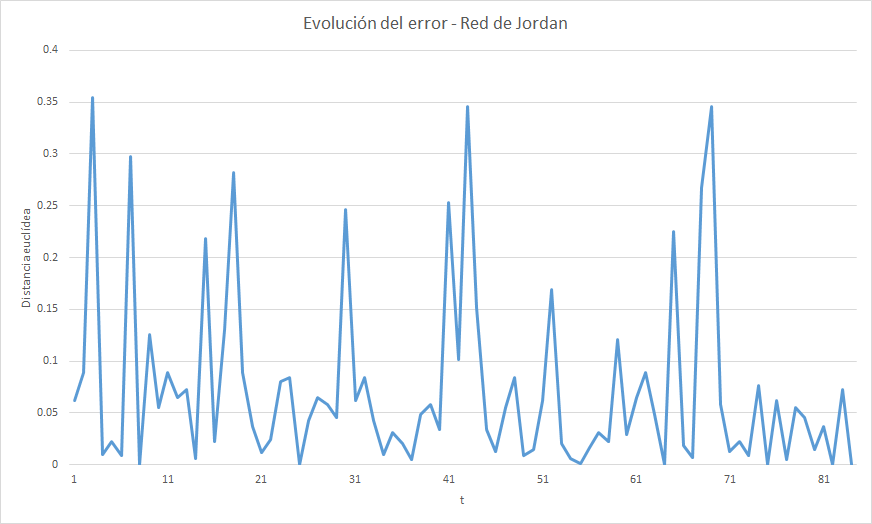
\includegraphics[width=1.0\textwidth]{red_jordan_error.png}
\end{figure}

En este caso, teniendo en cuenta que un valor predicho se consideraba acierto si el error era inferior a 0.05, podemos concluir que aproximadamente un 50\% de los valores predichos son aciertos.

\end{document}
